%---------- Terceiro Capitulo ----------
\chapter{Proposta}

A proposta desse projeto \'e desenvolver um aplicativo para dispositivos m\'oveis com sistema operacional Android, tendo como fun\c{c}\~ao principal o \sigla{RAA}{retroalimenta\c{c}\~ao auditiva atrasada}, ou seja, um aplicativo que consiga reproduzir a voz do usu\'ario simultaneamente com um pequeno atraso configur\'avel, num tom diferente tamb\'em configur\'avel. 

O atraso ser\'a medido em milissegundos, sendo poss\'ivel utilizar o intervalo entre 100 e 3000 milissegundos (0,1 e 3 segundos). A frequ\^encia ser\'a medida em Mega-hertz, possuindo as op\c{c}\~oes de 4 intervalos: 500, 1.000, 2.000 e 4.000 Mhz respectivamente.  Esses dados foram obtidos atrav\'es de uma pesquisa, onde participaram 20 indiv\'iduos com gagueira de 7 a 17 anos, resultando em uma diminui\c{c}\~ao estatisticamente significante na ocorr\^encia de bloqueios e repeti\c{c}\~oes de palavras em indiv\'iduos com gagueira sem altera\c{c}\~ao do processamento auditivo central, ou seja, sem altera\c{c}\~ao na capacidade que o sistema nervoso tem para traduzir as informa\c{c}\~oes enviadas pela audi\c{c}\~ao \cite{PICOLOTO2017}.

A finalidade dessas configura\c{c}\~oes que devem ser adaptadas para cada indiv\'iduo \'e simular o efeito coro, que nada mais \'e do que um efeito causado quando uma pessoa que possui gagueira, fala ou l\^e ao mesmo tempo que outra, trazendo melhorias significativas na fala \cite{Udemo2008}.


\section{Tecnologias e Ferramentas}
\begin{itemize}
	
	\item Java: utiliza-se como linguagem de programa\c{c}\~ao.
	
	\item Android Studio: utiliza-se como ambiente de desenvolvimento 		(\sigla{IDE}{Ambiente de Desenvolvimento Integrado}).

	\item Github: utiliza-se como reposit\'orio de armazenamento e controle de vers\~oes.
	
	\item Google Drive: utiliza-se como gerenciador de arquivos de texto, e planilhas.

	\item UML: utiliza-se como linguagem-padr\~ao para a elabora\c{c}\~ao da estrutura de projetos de \textit{software}.

	\item Astah: utiliza-se como ferramenta de modelagem \sigla{UML}{Linguagem Unificada de Modelagem}. 

\end{itemize}

\section{M\'etodo}

Uma alternativa para atender clientes e projetos de forma din\^amica, flex\'ivel e com produtividade elevada \'e a metodologia \textit{Agile}, ou \'agil em portugu\^es, que tem se consolidado ao longo dos \'ultimos anos com a utiliza\c{c}\~ao de uma abordagem de planejamento iterativa. O \textit{Scrum} \'e um \textit{framework} muito utilizado entre as metodologias \'ageis, especialmente pelo formato din\^amico como as etapas dos projetos s\~ao desenvolvidas \cite{Udacity2017}. 

Para o desenvolvimento do aplicativo descrito neste documento, utiliza-se uma metodologia incremental adaptada e baseada no \textit{Scrum}, seguindo alguns de seus conceitos mais importantes, como: 

\begin{itemize}
	
	\item \textit{Sprint}: s\~ao itera\c{c}\~oes, ciclos de desenvolvimento que come\c{c}am numa reuni\~ao de planejamento (\textit{Sprint Planning}) e terminam com a revis\~ao (\textit{Sprint Review}) e a retrospectiva (\textit{Sprint Retrospective}).
	
	\item \textit{Product Owner}: \'e o respons\'avel por definir prioridades a serem desenvolvidas em cada \textit{sprint} e fazer a intermedia\c{c}\~ao entre equipe de neg\'ocios e equipe de \textit{scrum}.
	
	\item \textit{Scrum Master}: respons\'avel por resolver impedimentos que possam prejudicar a equipe \textit{scrum}, e assegurar que todos sigam a metodologia proposta. 
	
	\item \textit{Sprint Planning}: reuni\~ao para planejar quais itens do \textit{backlog} do produto ser\~ao priorizados em determinada \textit{sprint}, que abrange determinado per\'iodo(1 at\'e 4 semanas).
	
	\item  \textit{Sprint Meeting Review}: Reuni\~ao de revis\~ao da \textit{sprint}, discutindo tudo que foi desenvolvido naquele ciclo. 
	
	\item \textit{Sprint Retrospective}: realizada ap\'os a reuni\~ao de revis\~ao e antes da reuni\~ao de planejamento, visa estabelecer poss\'iveis melhorias. 
		
\end{itemize}



\section{An\'alise e Desenvolvimento}

\subsection{Arquitetura}
Utiliza-se como arquitetura de desenvolvimento, a arquitetura de camadas do software Android, que \'e executado sobre um \textit{kernel} Linux. Os aplicativos Android s\~ao gravados na linguagem de programa\c{c}\~ao Java e s\~ao executados em uma \sigla{VM} {m\'aquina virtual} \cite{Ableson2009}.

A figura a seguir apresenta a maioria dos componentes da plataforma Android. 
\begin{figure}[H]
	\centering
	%\captionsetup{width=0.97\textwidth}
	\caption[Camadas do Software Android]{Camadas do Software Android. \label{fig:figurearquitetura}}
	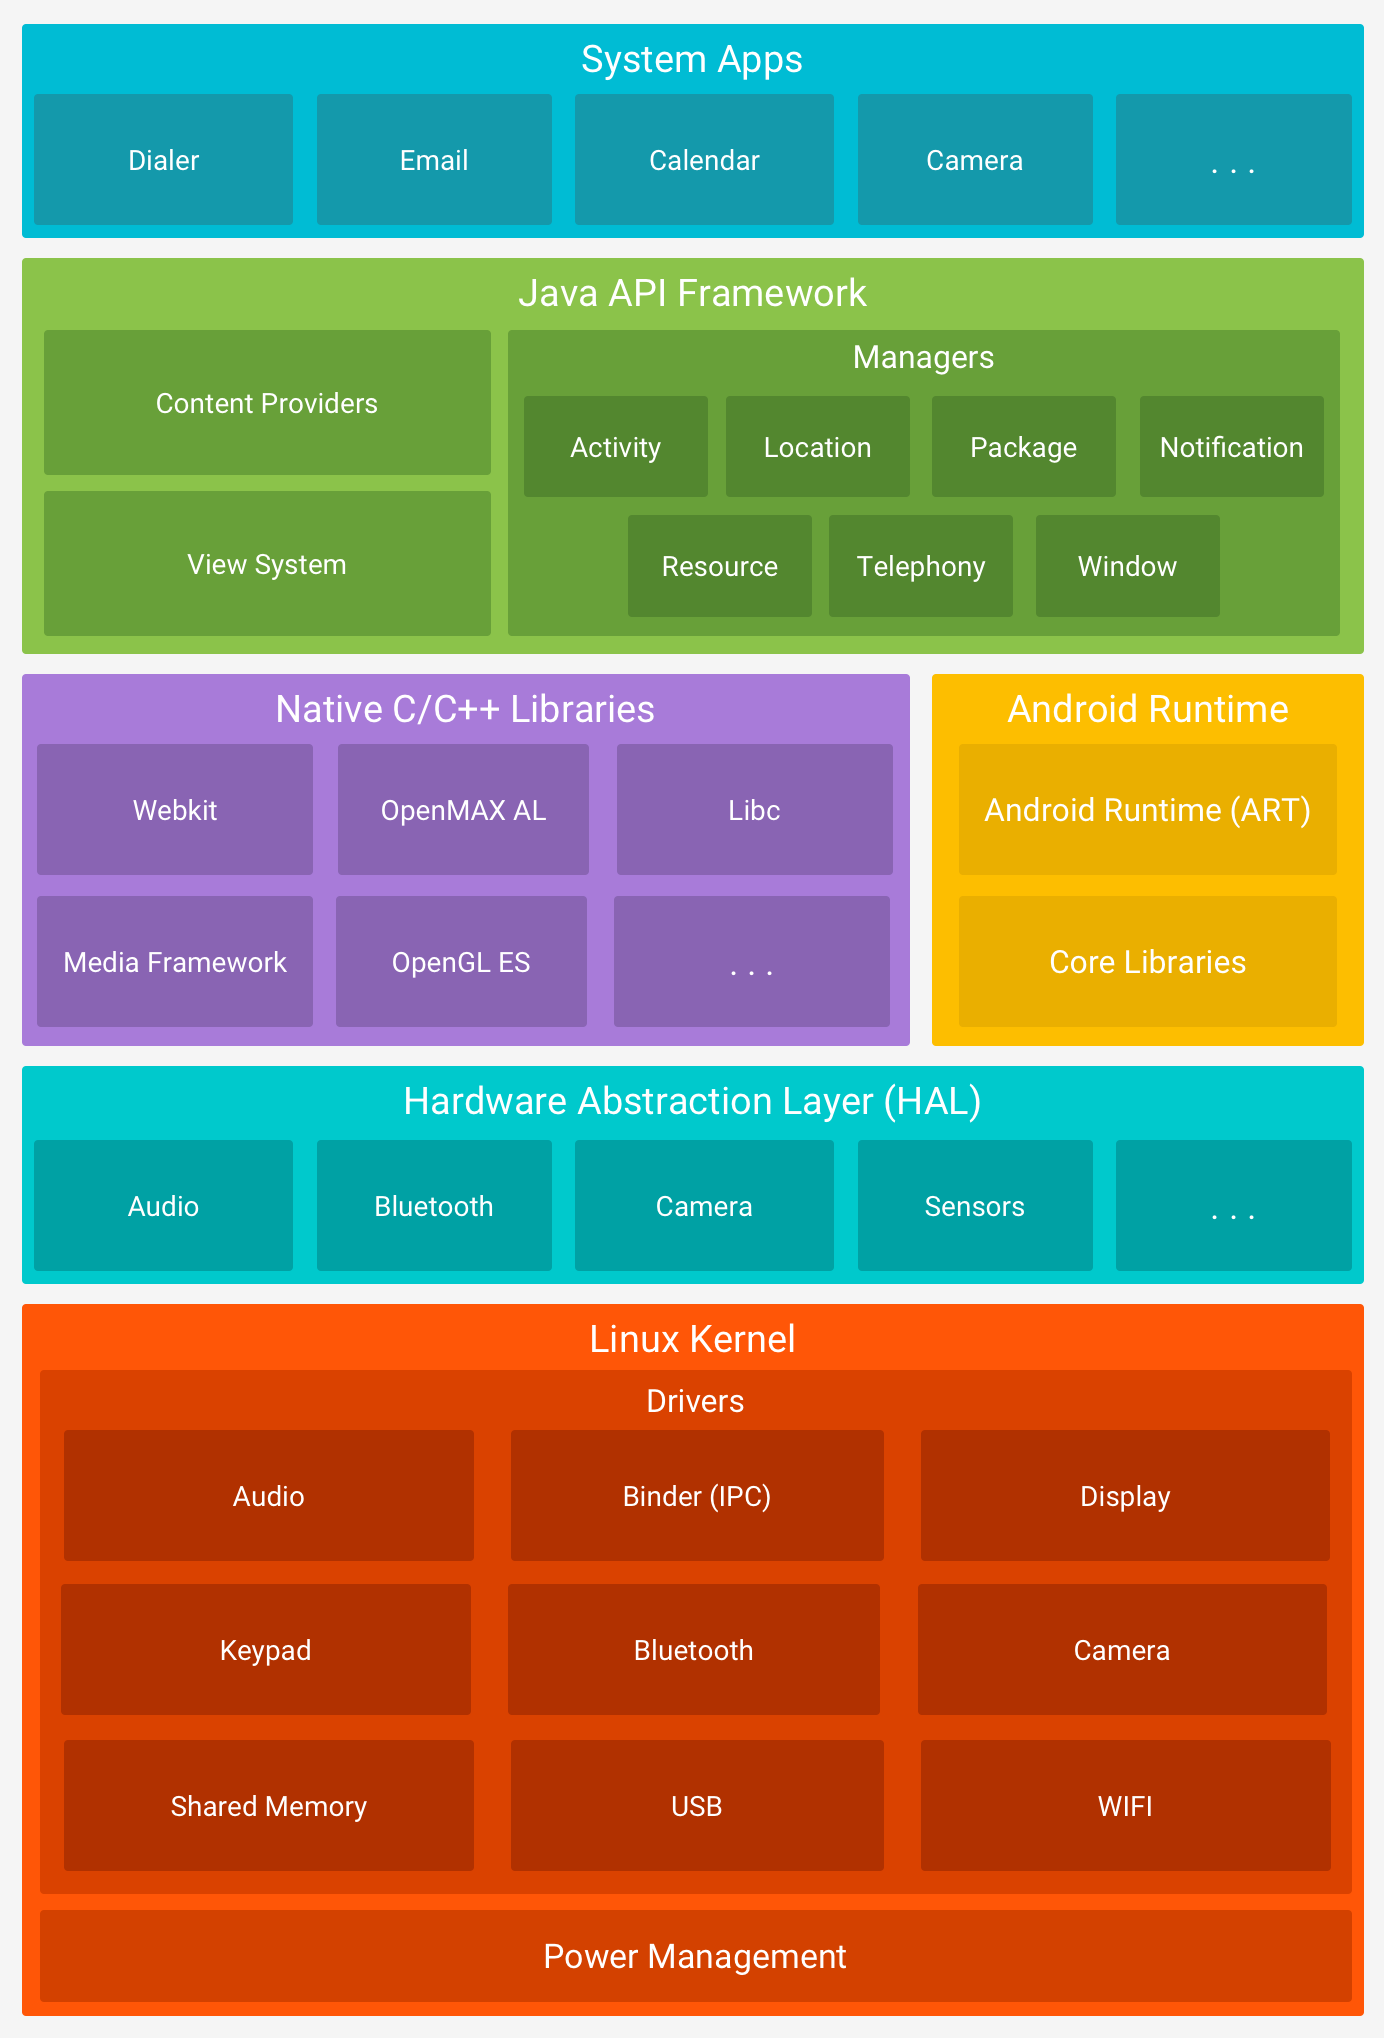
\includegraphics[height=15cm]{./Figuras/arquitetura_figure.png}% <- formatos PNG, JPG e PDF
	\fonte{\cite{Developers2018}}
\end{figure}


\subsection{Requisitos}

Nesta se\c{c}\~ao apresenta-se os requisitos do sistema, divididos em:
\begin{itemize}
	
	\item  Requisitos Funcionais (RF): apresentam as funcionalidades do sistema, ou seja, define oque o sistema far\'a. 
	
	\item Requisitos N\~ao-Funcionais (RNF): apresentam os atributos de qualidade para o sistema, ou seja, como o sistema far\'a determinada atividade, podendo ser categorizados em: usabilidade, desempenho, padr\~ao, etc \cite{Ventura2016}. 
	
\end{itemize}

A prioridade dos requisitos pode ser classificada em: 

\begin{itemize}
	
	\item Essencial: deve ser implementado para que o sistema funcione. 

	\item Importante: sem este requisito o sistema pode funcionar, mas n\~ao da maneira esperada.
	
	\item Desej\'avel: este tipo de requisito n\~ao compromete o funcionamento do sistema.
	
\end{itemize}

\begin{table}[H]
	\caption{Requisitos Funcionais}\label{tab:reqfuncionais}
	\centering
	\begin{tabular}{|p{1.0cm}|p{8.0cm}|p{2.0cm}|p{2.5cm}|}
		\hline
		\textbf{Id} & \textbf{Descri\c{c}\~ao} & \textbf{Prioridade} & \textbf{Requisitos Relacionados}\\
		\hline
		RF01 & O aplicativo deve permitir ao usu\'ario editar as prefer\^encias de utiliza\c{c}\~ao do aplicativo, como tipo de fone utilizado, altura do volume, frequ\^encia e delay. & Essencial & RF02 - RF04\\
		\hline
		RF02 & O aplicativo deve permitir ao usu\'ario iniciar e interromper a simula\c{c}\~ao do efeito coro. & Essencial & N/A \\
		\hline
		RF03 & O aplicativo deve manter salva as prefer\^encias de utiliza\c{c}\~ao. & Importante & RF01 - RF04\\
		\hline
		RF04 & O aplicativo deve fornecer a op\c{c}\~ao de um tutorial em seu primeiro uso. & Importante & N/A\\
		\hline
		RF05 & O aplicativo deve permitir a utiliza\c{c}\~ao de fone \textit{bluetooth}. & Importante & RF01 - RF002\\
		\hline
		RF06 & O aplicativo deve permitir ao usu\'ario uma op\c{c}\~ao de n\~ao receber liga\c{c}\~oes, enquanto o aplicativo estiver executando a simula\c{c}\~ao do efeito coro. & Desej\'avel & RF01\\
		\hline
		RF07 & O aplicativo deve conter uma tela de ajuda, onde existir\'a informa\c{c}\~oes sobre a utiliza\c{c}\~ao do aplicativo. & Desej\'avel & RF03\\
		\hline
		RF08 & O aplicativo deve permitir visualizar o registro de vezes em que o usu\'ario utilizou o aplicativo. & Desej\'avel & RF02\\
		\hline
		RF09 & O aplicativo deve permitir modos personalizados, como a cria\c{c}\~ao de: modo casa, modo apresenta\c{c}\~ao, modo tutorial, entre outros. Onde cada modo possui prefer\^encias pr\'e-definidas. & Desej\'avel & RF01-RF03\\
		\hline	
	\end{tabular}
	\fonte{O Autor.}	
\end{table}


\begin{table}[H]
	\caption{Requisitos N\~ao-Funcionais}\label{tab:reqnaofuncionais}
	\centering
	\begin{tabular}{|p{1.0cm}|p{5.0cm}|p{2.5cm}|p{2.0cm}|p{2.5cm}|}
		\hline
		\textbf{Id} & \textbf{Descri\c{c}\~ao}& \textbf{Categoria} & \textbf{Prioridade} & \textbf{Requisitos Relacionados}\\
		\hline
		RNF01 & O aplicativo deve ser desenvolvido para a plataforma Android. & Compatibilidade & Essencial & RFN03\\
		\hline
		RNF02 & O usu\'ario do aplicativo deve ser capaz de usufruir das suas funcionalidades com no m\'aximo 1 minuto de utiliza\c{c}\~ao. & Usabilidade & Importante & RNF04 \\
		\hline
		RNF03 & O aplicativo deve ser implementado na linguagem de programa\c{c}\~ao JAVA. & Implementa\c{c}\~ao  & Importante & RNF01\\
		\hline
		RNF04 & A interface do aplicativo deve ser simples, com no m\'aximo 5 bot\~oes, ou controladores (Aumentar ou diminuir a frequ\^encia e o \textit{delay}, bot\~ao iniciar/desligar, e op\c{c}\~ao de configura\c{c}\~oes). & Usabilidade & Desej\'avel & RNF02\\
		\hline
	\end{tabular}
	\fonte{O Autor.}
\end{table}


\subsection{Diagrama de Classes}

Apresenta-se o diagrama de classes, uma representa\c{c}\~ao da estrutura e rela\c{c}\~oes das classes que servem de modelo para objetos \cite{Tybel2017}.

\begin{figure}[H]
	\centering
	%\captionsetup{width=0.97\textwidth}
	\caption[Diagrama de Classes]{Diagrama de Classes. \label{fig:diagramadeclasses}}
	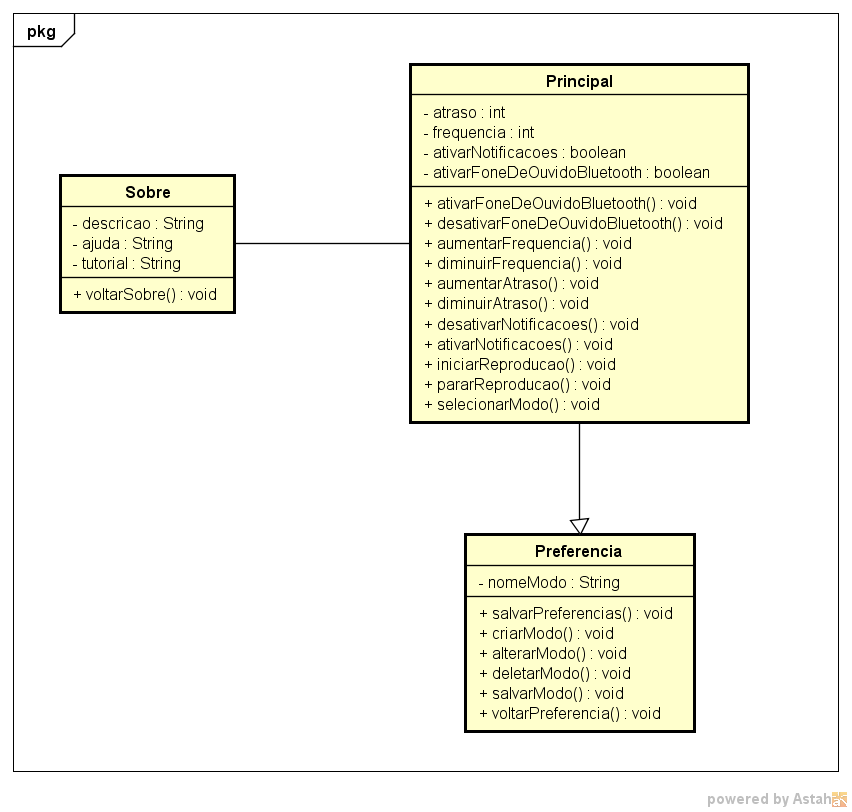
\includegraphics[height=15cm]{./Figuras/class_diagram.png}% <- formatos PNG, JPG e PDF
	\fonte{O Autor.}
\end{figure}

\subsection{Diagrama de Casos de Uso}

Apresenta-se o diagrama de casos de uso, documentando o que o sistema faz do ponto de vista do usu\'ario, ou seja, descreve as principais funcionalidades do sistema e a intera\c{c}\~ao dessas funcionalidades com os usu\'arios do mesmo sistema \cite{Ribeiro2012}.

\begin{figure}[H]
	\centering
	%\captionsetup{width=0.97\textwidth}
	\caption[Diagrama de Casos de Uso]{Diagrama de Casos de Uso. \label{fig:diagramadecasosdeuso}}
	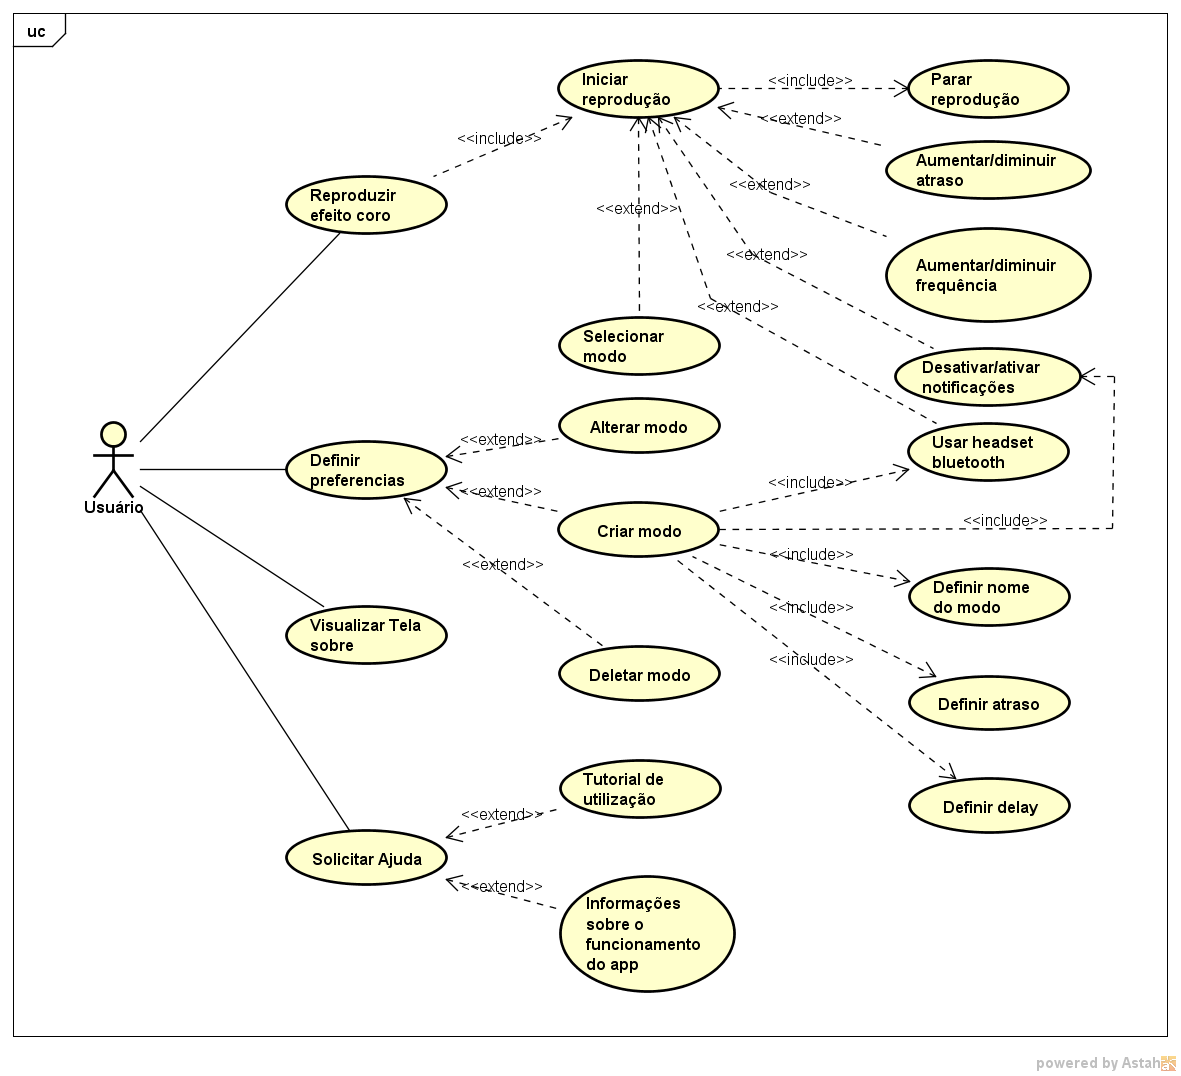
\includegraphics[height=15cm]{./Figuras/usecase_diagram.png}% <- formatos PNG, JPG e PDF
	\fonte{O Autor.}
\end{figure}

\subsection{Diagrama de Atividades}

Apresenta-se o diagrama de atividades, com o objetivo de mostrar o fluxo de atividades em um \'unico processo, especificando o comportamento do software do ponto de vista funcional \cite{Ventura2016a}. 
\begin{figure}[H]
	\centering
	%\captionsetup{width=0.97\textwidth}
	\caption[Diagrama de Atividades]{Diagrama de Atividades. \label{fig:diagramadeatividades}}
	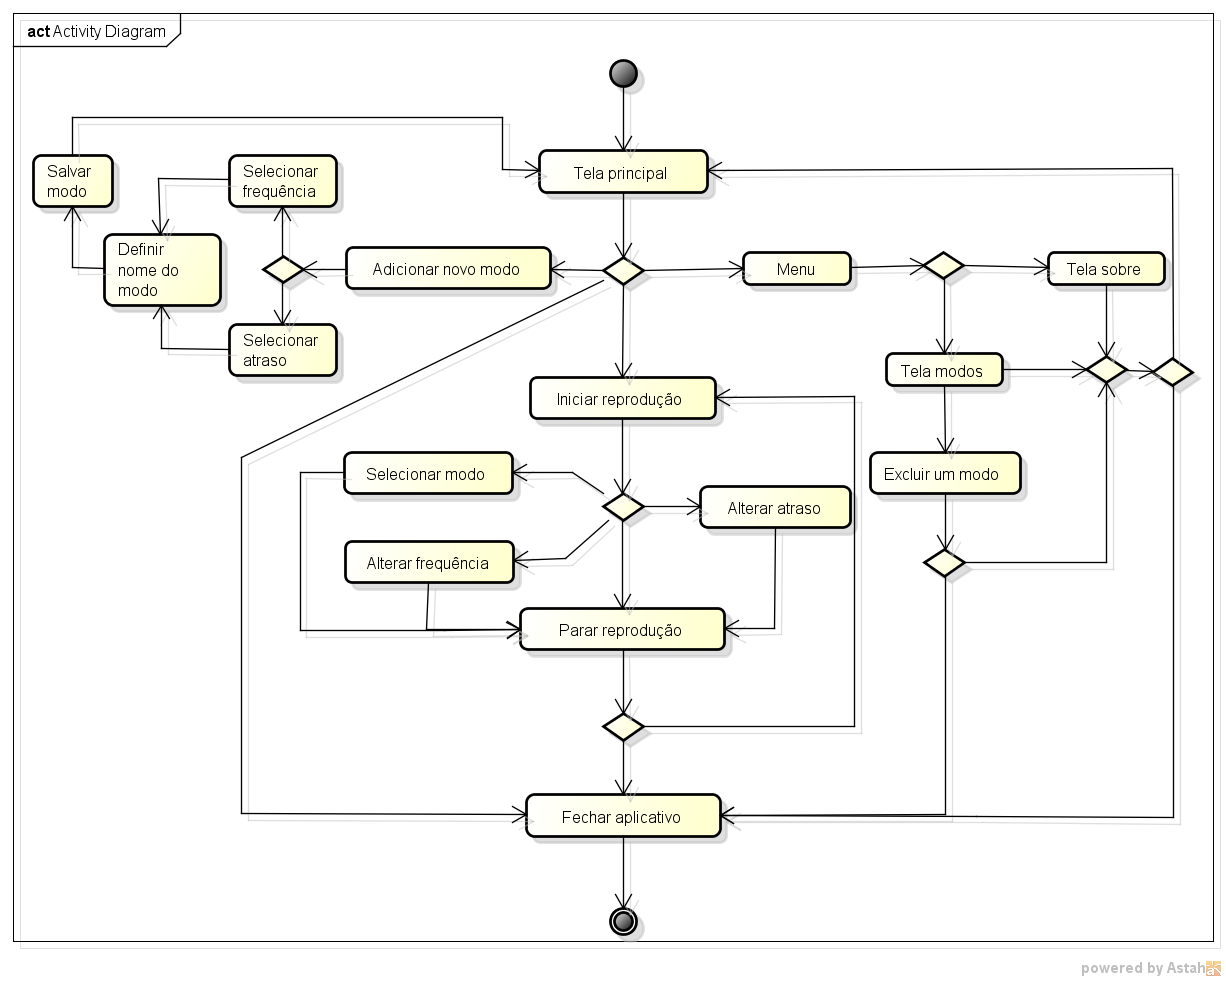
\includegraphics[height=13cm]{./Figuras/activity_diagram.png}% <- formatos PNG, JPG e PDF
	\fonte{O Autor.}
\end{figure}

\section{Prot\'otipos de Tela}

Apresenta-se os prot\'otipos de tela do sistema. 

\begin{itemize}
	\item Tela Inicial: Nesta tela o usu\'ario tem acesso a todas as funcionalidades do sistema, al\'em de iniciar a simula\c{c}\~ao do efeito coro, ele pode ajustar o atraso e a frequ\^encia de acordo com suas prefer\^encias, tamb\'em tem a op\c{c}\~ao de ativar e desativar a fun\c{c}\~ao de utilizar \textit{headset bluetooth}, localizado no canto superior esquerdo da tela, juntamente com desativar as notifica\c{c}\~oes marcando o \textit{combobox} "Desativar notifica\c{c}\~oes. Desta tela tamb\'em existe a op\c{c}\~ao de navegar entre as telas "Sobre" e "Prefer\^encias", selecionando o \'icone referente a cada tela localizados no canto superior direito.
	\begin{figure}[H]
		\centering
		%\captionsetup{width=0.97\textwidth}
		\caption[Prot\'otipo Tela Inicial]{Prot\'otipo Tela Inicial. \label{fig:prototipotelainicial}}
		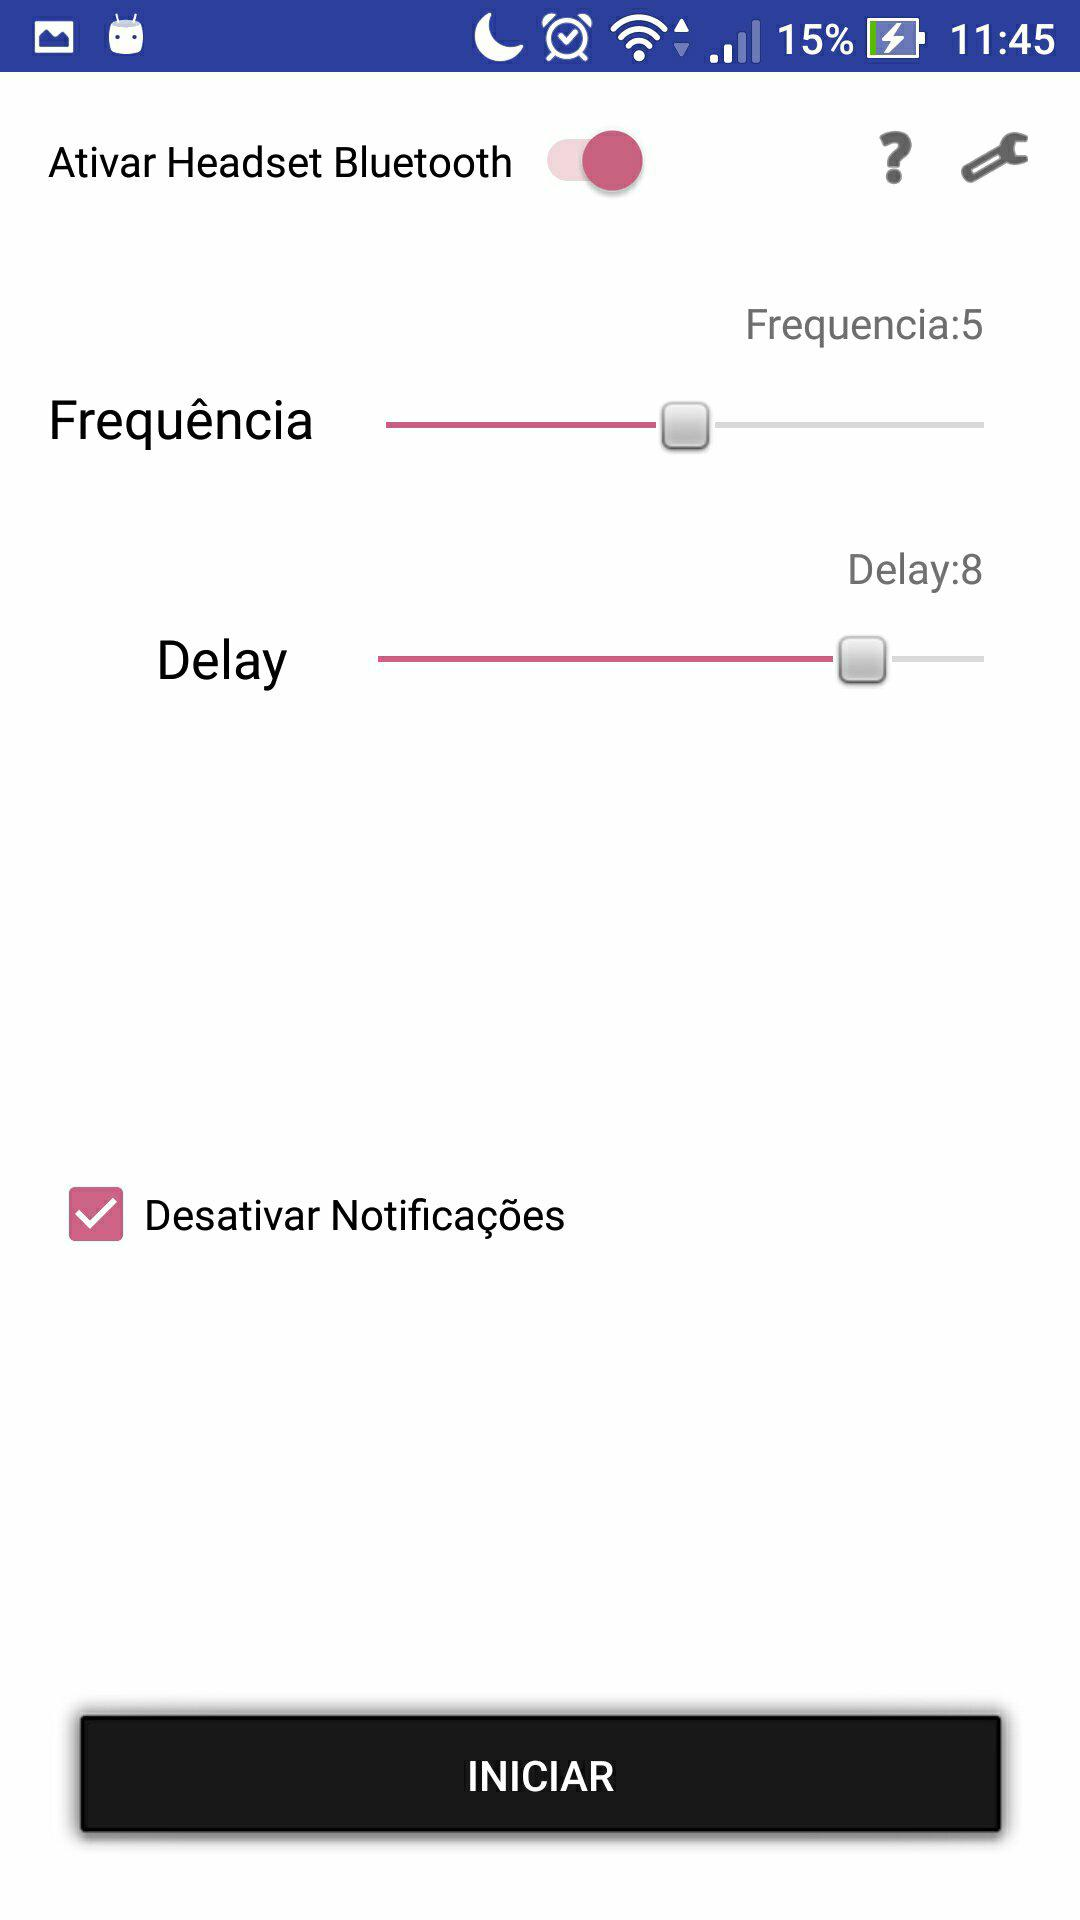
\includegraphics[height=13cm]{./Figuras/prototipo_telainicial.jpg}% <- formatos PNG, JPG e PDF
		\fonte{O Autor.}
	\end{figure}
	
	\item Tela Prefer\^encias: Nesta tela o usu\'ario pode criar, alterar, ou excluir um modo, adicionando o atraso e frequ\^encia desejados, al\'em de selecionar as op\c{c}\~oes de ativar/desativar \textit{headset bluetooth} e notifica\c{c}\~oes;
	\begin{figure}[H]
		\centering
		%\captionsetup{width=0.97\textwidth}
		\caption[Prot\'otipo Tela Prefer\^encias]{Prot\'otipo Tela Prefer\^encia. \label{fig:prototipotelapreferencias}}
		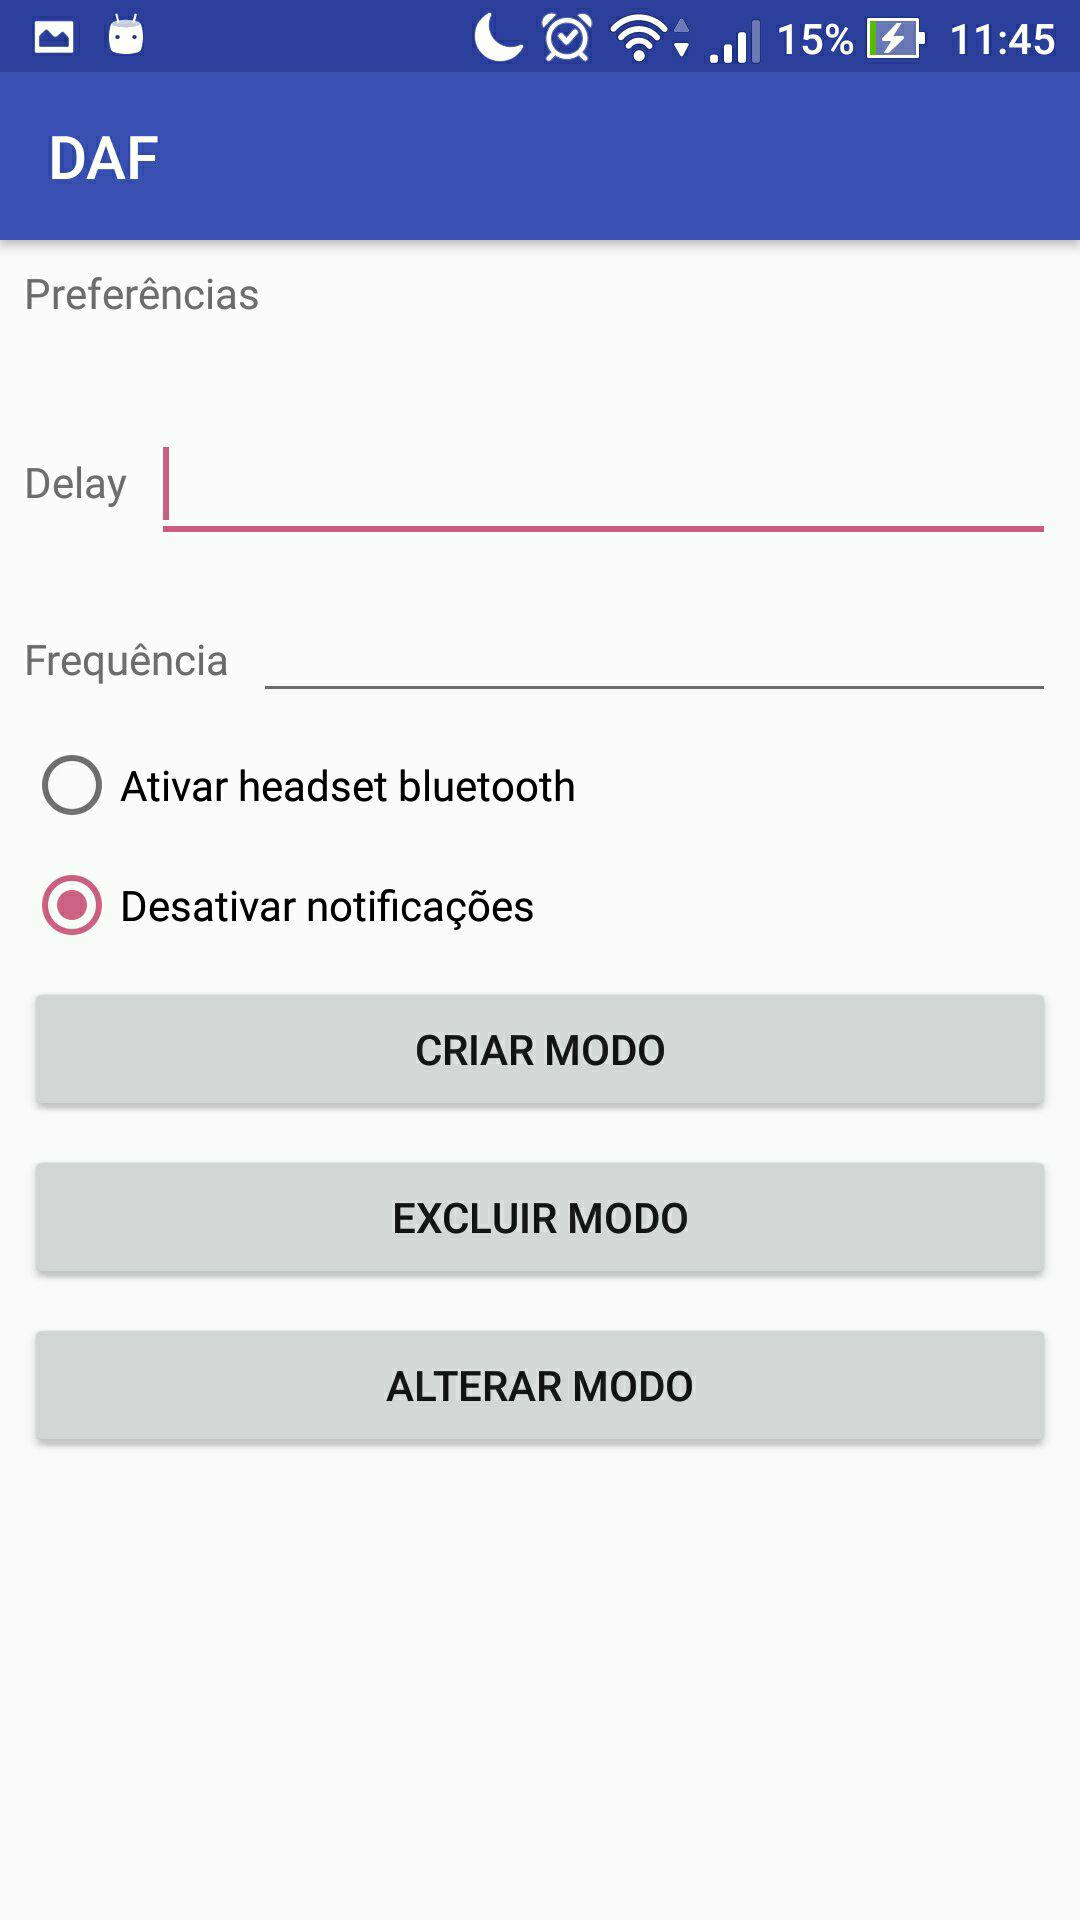
\includegraphics[height=13cm]{./Figuras/prototipo_telapreferencias.jpg}% <- formatos PNG, JPG e PDF
		\fonte{O Autor.}
	\end{figure}

	\item  Tela Sobre: Nesta tela o usu\'ario encontra informa\c{c}\~oes sobre o aplicativo, assim como informa\c{c}\~oes sobre o funcionamento do aplicativo e um tutorial de ajuda. 
	\begin{figure}[H]
		\centering
		%\captionsetup{width=0.97\textwidth}
		\caption[Prot\'otipo Tela Sobre]{Prot\'otipo Tela Sobre. \label{fig:prototiposobre}}
		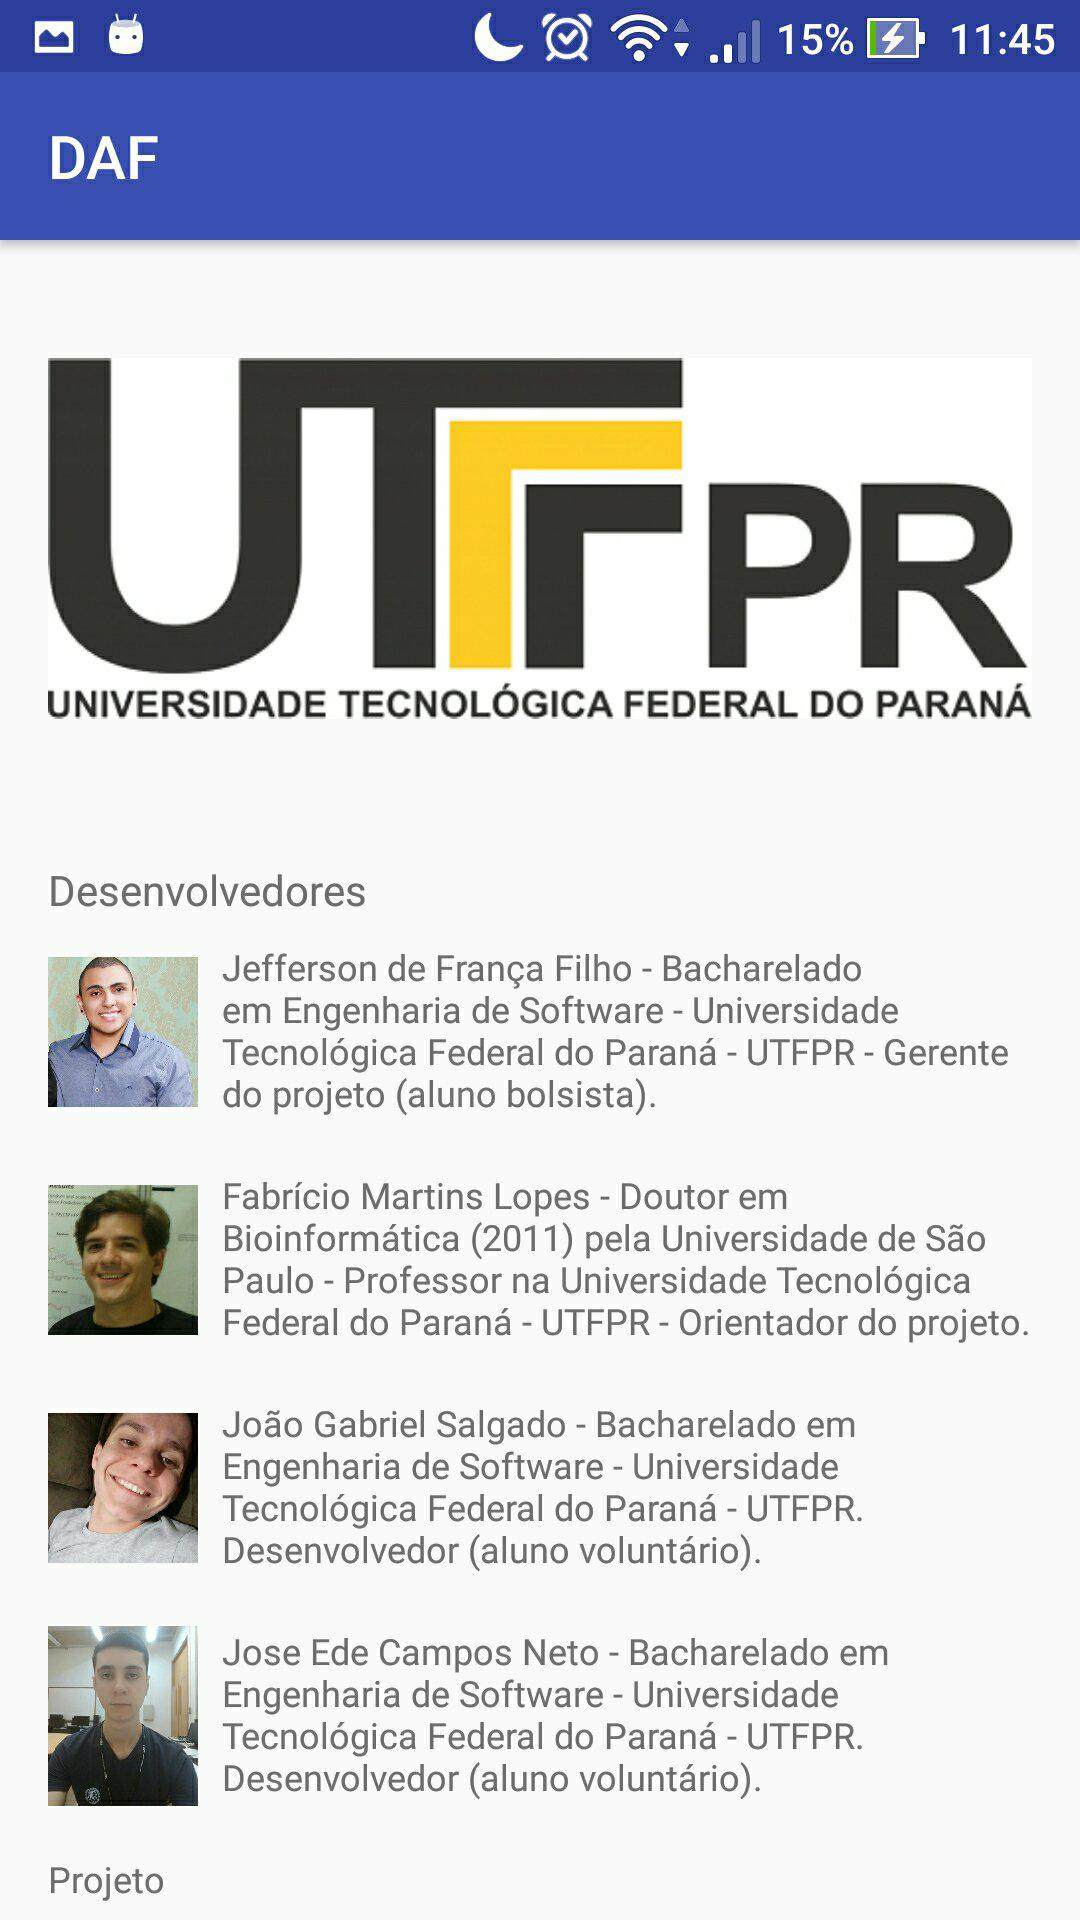
\includegraphics[height=13cm]{./Figuras/prototipo_sobre.jpg}% <- formatos PNG, JPG e PDF
		\fonte{O Autor.}
	\end{figure}
\end{itemize}

\section{Cronograma}

Apresenta-se o cronograma, determinando todas as atividades do processo de desenvolvimento do software, com o per\'iodo definido de 10 meses, definido de acordo com o programa "Protagonismo Estudantil", projeto ao qual a proposta do aplicativo apresentado neste documento foi contemplado com bolsa remunerada, tendo in\'inicio em outubro de 2017. 

\begin{table}[H]
	 \caption{Cronograma de atividades}
	 \label{tab:cronograma}
	 \begin{center}
		  \begin{tabular}{|l||c|c|c|c|c|c|c|c|c|c|}
			    \hline
			    \multicolumn{1}{|c||}{Fase} 	&Out     			&Nov     			&Mar     			&Abr   			&Mai 				&Jun 			&Jul 			&Ago			&Set				&Out\\ \hline
			    Levantamento de requisitos 	& $\bullet$  	&           	&          		&         		&  				&  			&  			&			&	 			&\\
			    An\'alise de requisitos    	& $\bullet$     &  				& 				&         		&  				&  			&  			& 			&				&\\
			    Projeto   				   	&           	&$\bullet$    	& 				& 				&  				&  			&  			& 			&				&\\
			    Implementa\c{c}\~ao   	   	&           	&          		&$\bullet$   	&$\bullet$    	&$\bullet$		&$\bullet$ 	&$\bullet$ 	&			&				&\\
			    Testes    				   	&           	&           	& 				&$\bullet$ 		&$\bullet$ 		&$\bullet$ 	&$\bullet$  &$\bullet$	&				&\\
			    Implanta\c{c}\~ao    	   	&           	&           	&				& 				&  				&  			&  			&		 	&$\bullet$		&\\
			    Divulga\c{c}\~ao 		   	& 				& 				&				&				&				& 			&			& 			& 				&$\bullet$\\
			    \hline
			  \end{tabular}
		 \vspace{8pt} %%%% Deve ser acrescentado para que haja espaço entre o final da tabela e a fonte.
		  \fonte{O Autor.}
		 \end{center}
\end{table}
